\documentclass[conference]{IEEEtran}
\IEEEoverridecommandlockouts
% The preceding line is only needed to identify funding in the first footnote. If that is unneeded, please comment it out.
\usepackage{cite}
\usepackage{amsmath,amssymb,amsfonts}
\usepackage{algorithmic}
\usepackage{url}
%\usepackage[authoryear]{natbib}
%\usepackage{filecontents}
\usepackage{graphicx}
\graphicspath{ {images/} }
\usepackage{textcomp}
\usepackage{xcolor}
\usepackage{stackengine}
\stackMath
\def\BibTeX{{\rm B\kern-.05em{\sc i\kern-.025em b}\kern-.08em
    T\kern-.1667em\lower.7ex\hbox{E}\kern-.125emX}}
\begin{document}

\title{Resource Access Protocols\\
{\footnotesize }
\thanks{University of Applied Science Hamm-Lippstadt}
}

\author{\IEEEauthorblockN{1\textsuperscript{st} Sheikh Muhammad Adib Bin Sh Abu Bakar}
\IEEEauthorblockA{\textit{University of Applied Science Hamm-Lippstadt} \\
\textit{B.Eng. Electronic Engineering}\\
Lippstadt, Germany \\
sheikh-muhammad-adib.bin-sh-abu-bakar@stud.hshl.de}

}

\maketitle
\begin{abstract}

In hard real time system, it is important to ensure every single task not only to be successfully executed but to produce the right value on the right time. Thus, scheduling algorithm play a big role in handling various of task, either statically or dynamically. It is common in real time system environment, some tasks share the same resource, which is one of the complicated part in concurrent operating system. Any concurrent operating system should utilize proper synchronization to assure mutual exclusion among competing activities, in order to ensure the predictability of the system, which is important in oder to produce reliable system especially when safety is a crucial part. This is why resource access protocol one of the important topic in building a real time system. In this research paper, various of resource access protocol for uni-processor that are developed under fixed priority assignment will be explained. So, it will be clear for us which protocol should be implemented based on the environment that we are working on. To ensure this paper is easy to understand, I also include basic information about real time system before going deep into resource access protocol.
\end{abstract}



\begin{IEEEkeywords}
real time system, resource access protocol 
\end{IEEEkeywords}

\subsection{Real Time System}


\subsection{Characteristics}

%Real Time System
%predictibility
%application domain
%important aspect
%flow

%task

%scheduling
%classification
%-preemtion
%-non-preemtion
%-dynamic
%-static
%-online
%periodic
%schedubility test

%constraint
%-timming
%-resource
%share resource
%problem
%solution (resource constarint)

\section{Background}
In this section, we will describe the concept and terms that are dominant in this research paper.

\subsection{Task}

According to \cite{b4}- "a Task is a sequence of instructions that, in the absence of other activities, is continuously executed by the processor until completion."

Task, thread, job and process  are the basic component in task scheduling. At the level of scope of this paper, the term process and thread have the same definition as task. 

An example of a task could be writing or reading a variable's value. Some task have its instance called Job as defined in \cite{b4}-"Job is an instance of a task executed on a specific input data". 

Next I will explain how tasks are executed.


\subsection{Scheduling Policy and Scheduling Algorithm }


In real time system, more than one task that are concurrent, are handled even in system with uni-processor. To realize it,  the task are executed in order using a defined algorithm called scheduling algorithm. For that reasons many scheduling algorithm have been proposed such as Earliest Deadline First, The Earliest Deadline Late serve and many more. The task is ordered by assigning their priority through set of predefined criterion called scheduling policy.\cite{b5}

Considering that the schedule algorithm handles more than one task, now we will extend the definition of a task to correspond to their state as listed in the list below.

\begin{itemize}
\item A task that could potentially execute on the CPU can be either in execution (if it has been selected by the scheduling algorithm) or waiting for the CPU (if another task is executing)\cite{b5}.

\item A task that can potentially execute on the processor, independently of its actual availability, is called an active task\cite{b5}.

\item A task waiting for the processor is called a ready task, whereas the task in execution is called a running task\cite{b5}.

\item All ready tasks waiting for the processor are kept in a queue, called ready queue\cite{b5}.

\end{itemize}

Scheduling Algorithms are built to solve a curtain problem for a curtain environment. Means that they can be classified base on their characteristic. The classification of the algorithm will be explained in the next subtopic.

\subsection{Classification of Scheduling Algorithms}

In this subtopic, we will only focus on important classification of scheduling algorithm that are related to the scope of this paper, which is resource access protocols that will be discussed in resource access protocol section. 

\begin{itemize}
\item Preemptive: running task can be interrupted at any time\cite{b5}.
\item Non-preemptive: a task, once started, is executed until completion\cite{b5}.
\item Static: scheduling decisions are based on fixed parameters (off-line)\cite{b5}.
\item Dynamic: scheduling decisions are based on parameters that change during system evolution\cite{b5}.
\item Off-line : Scheduling algorithm is performed on the entire task set before start of system. Calculated schedule is executed by dispatcher\cite{b5}. 
\item On-line : scheduling decisions are taken at run-time every time a task enters or leaves the system\cite{b5}.
\item Optimal : the algorithm minimizes some given cost function, alternatively : it may fail to meet a deadline only if no other algorithm of the same class can meet it\cite{b5}.
\item Heuristic : algorithm that tends to find the optimal schedule, but does not guarantee to find it\cite{b5}.
\end{itemize}

In real time system not only the characteristic of algorithm are matter but also the characteristics  of task that being handle by scheduling algorithm, such as periodic and aperiodic that will be discussed in the next subtopic.

\subsection{Periodic and Aperiodic Task}

A task can be periodic or aperiodic, base on the way it is activated. Their definition is listed below:
\begin{itemize}
\item Periodic Task: a task in which jobs are activated at regular intervals of time, such that the activation of consecutive jobs is separated by a fixed interval of time, called the task period\cite{b4}.
\item Aperiodic Task: a task in which jobs may be activated at arbitrary time intervals\cite{b4}.
\end{itemize}

The resource access protocol, which we shall cover later, only handles periodic tasks. A periodic task is depicted in Figure \ref{fig:periodic}. As previously stated, a scheduling algorithm is used to handle many tasks by executing them in the order of their priority. The constraint they have influences their priority. Following that, I will go through some of the most important task constraints.

\begin{figure}[ht]
    \centering
    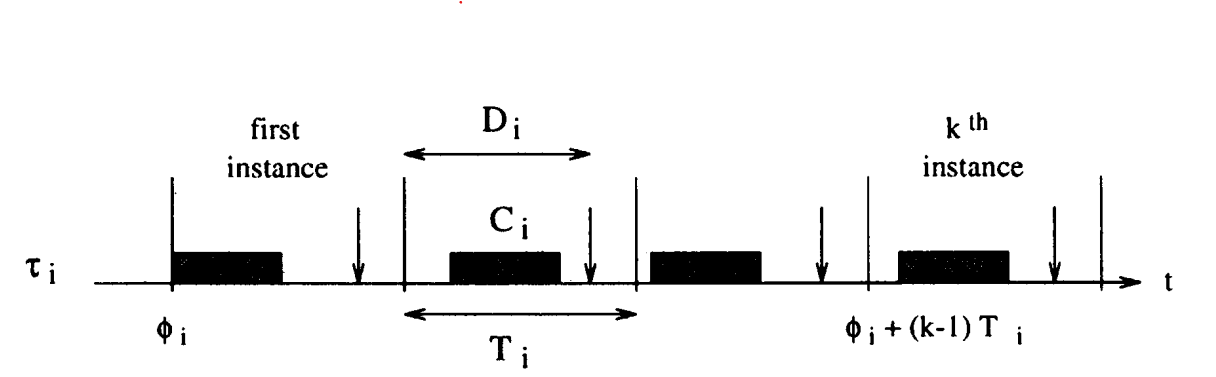
\includegraphics[width=0.5\textwidth]{periodic}
    \caption{periodic task \cite{b5}}
    \label{fig:periodic}
\end{figure}

\subsection{Task Constraint}

Task constraints are rules that are used by the scheduling algorithm to set  priority for each task. There are 3 main type of task constraint, and they are:

\begin{itemize}
\item Timing constraint
\item Precedence constraint
\item Resource constraint
\end{itemize}

Next we will explain more detail about timing constraint and resource constraint and how they are related to this paper topic. Precedence constraint is not covered in this paper. 

\subsubsection{Timing Constraint}

One of the timing constraint that are essential in this paper is deadline. There is two type of deadline:
\begin{itemize}
\item Relative Deadline: the longest interval of time within which any job should complete its execution\cite{b4}.
\item Absolute Deadline (of a job): the time at which a specific job should complete its execution\cite{b4}.
\end{itemize}

If concurrent tasks are not adequately managed, a task or job's deadline may be missed. As a result, we must make certain that our real-time system is well-predicted. This is why, in order to overcome the problem of system predictability, we have other constraints, such as resource constraint, which will be discussed in the following subsection. We may divide real-time systems into three groups based on their timing constraint, as follows:

\begin{itemize}
\item Hard Real Time System - failed to meet the deadline can cause catastrophic event 
\item Soft Real Time System - failed to meet the deadline only cause the degradation of the system 
\item Firm Real Time System - failed to meet the deadline only cause the production of useless output 
\end{itemize}
Hard real time is the main focus in this research paper.

\subsubsection{Resource Constraint}

As mentioned before, another important constraint related to this topic is resource constraint. First, we need to understand what resource means in this paper.

According to \cite{b5} - "resource is any software structure that can be used by the process to advance its execution. Typically, a resource can be a data structure, a set of variables, a main memory area, a file, a piece of program, or a set of registers of a peripheral device. A resource dedicated to a particular process is said to be private, whereas a resource that can be used by more tasks is called a shared resource. A shared resource protected against concurrent accesses is called an exclusive resource."


Resource constraint that we are focus on is the mechanism that avoid more than one concurrent tasks to access an exclusive resource at the same time. ``Fig. \ref{fig:Two_tasks_sharing}'' shows an example of resource, R that holding the value $x$ and $y$ and two tasks $\tau_{W}$ and $\tau_{D}$ with their critical sections. In general, concurrent tasks are not allowed to access shared resources at the same time to avoid data inconsistency, as illustrated in ``Fig. \ref{fig:Example_of_schedule_creating_data_inconsistency}''. Now, the value of $x$ and $y$ in critical section of $\tau_{D}$ is 4 and 2 instead of 4 and 8.

\begin{figure}[ht]
    \centering
    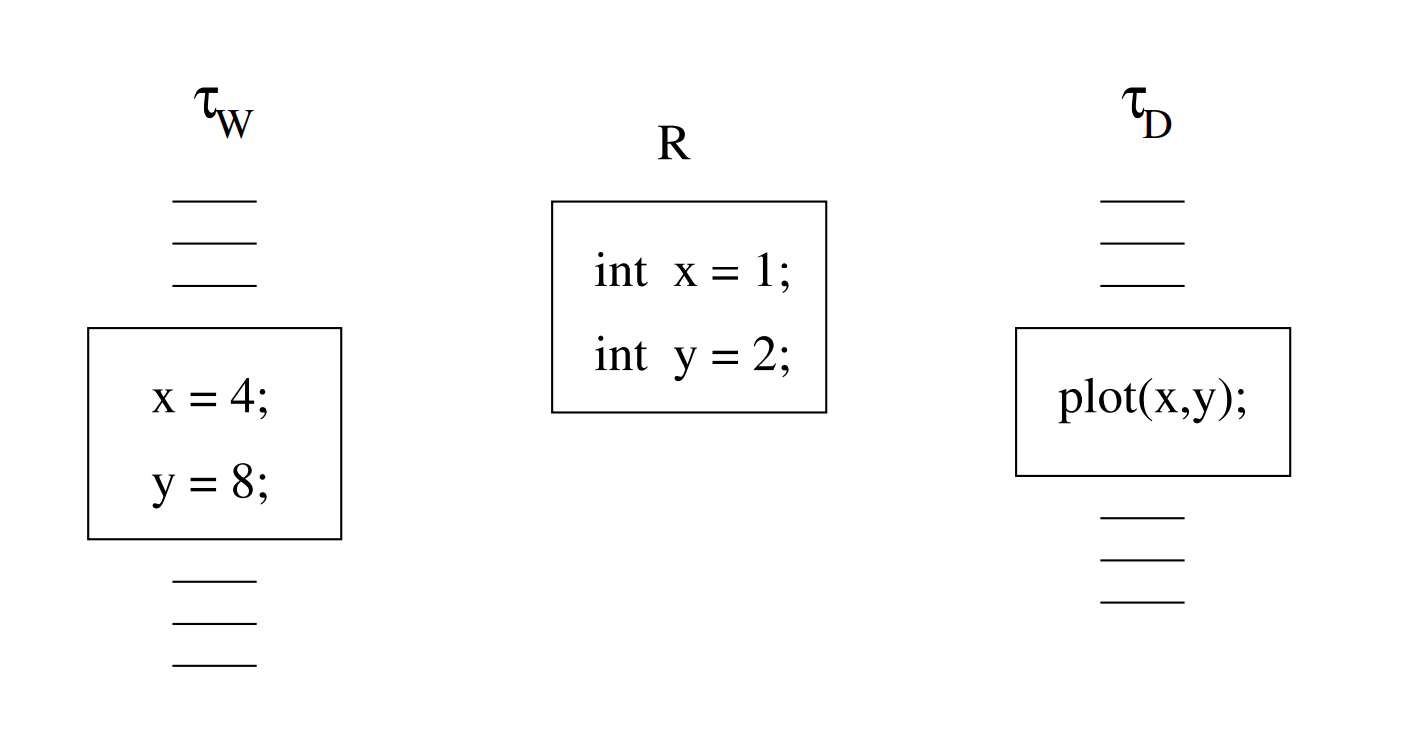
\includegraphics[width=0.4\textwidth]{Two_tasks_sharing}
    \caption{ Two tasks sharing a buffer with two variables. \cite{b5}}
    \label{fig:Two_tasks_sharing}
\end{figure}

\begin{figure}[ht]
    \centering
    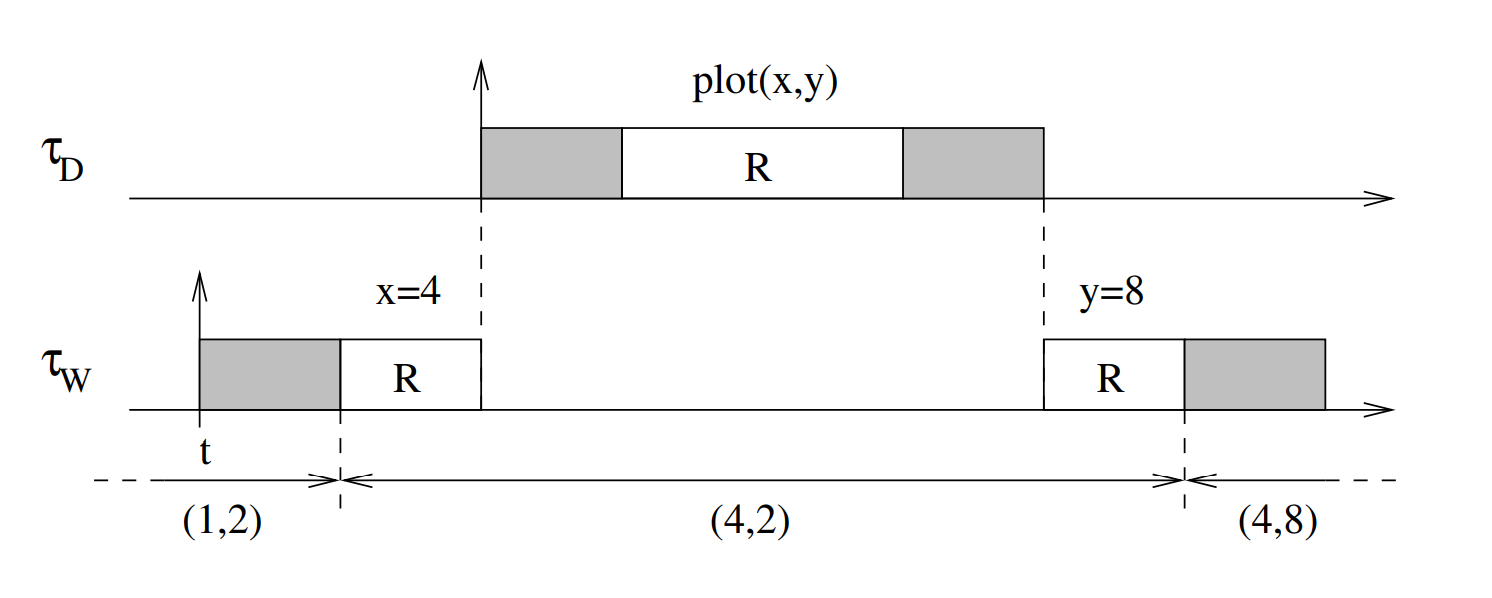
\includegraphics[width=0.5\textwidth]{Example_of_schedule_creating_data_inconsistency}
    \caption{Example of schedule creating data inconsistency. \cite{b5}}
    \label{fig:Example_of_schedule_creating_data_inconsistency}
\end{figure}

Various synchronization mechanisms, such as \textit{semaphore}, were devised to prevent this problem. Each critical section in this mechanism must start with wait(s) primitive and end with signal(s) primitive, where s is a binary semaphore, as shown in ``Fig. \ref{fig:Structure}'', and the state of a task may be extended thanks to this mechanism, as shown in ``Fig. \ref{fig:state}''. If another job is presently using the resource, the task will be unable to access it until the signal(s) is executed. As seen in ``Fig. \ref{fig:semaphore}'', this approach can assure data consistency. For the sake of simplicity, we will refer to exclusive resources as "resources" throughout this work.

\begin{figure}[ht]
    \centering
    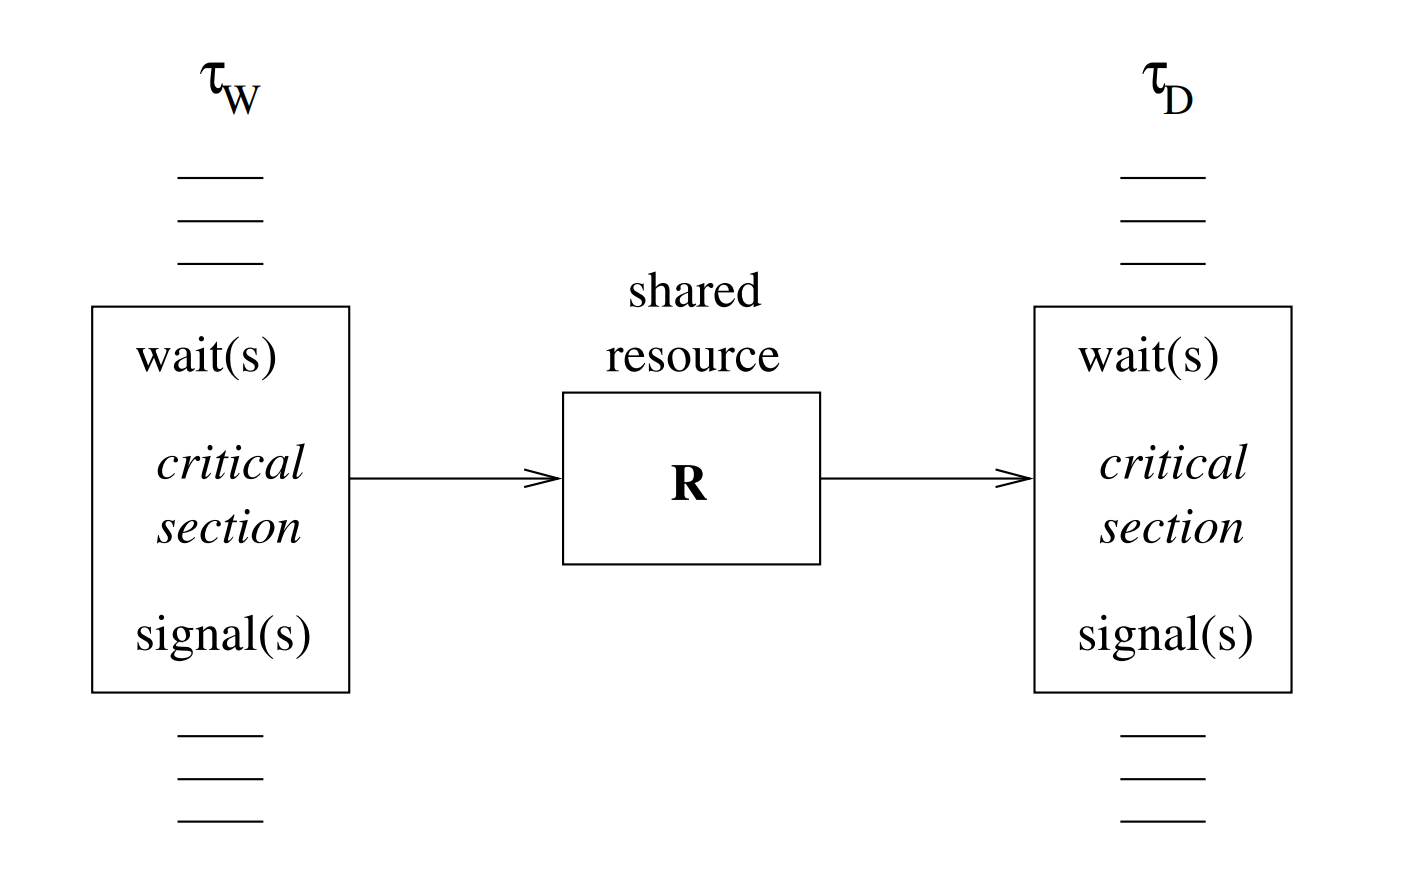
\includegraphics[width=0.4\textwidth]{Structure}
    \caption{Structure of two tasks that share a mutually exclusive resource protected by
a semaphore. \cite{b5}}
    \label{fig:Structure}
\end{figure}


\begin{figure}[ht]
    \centering
    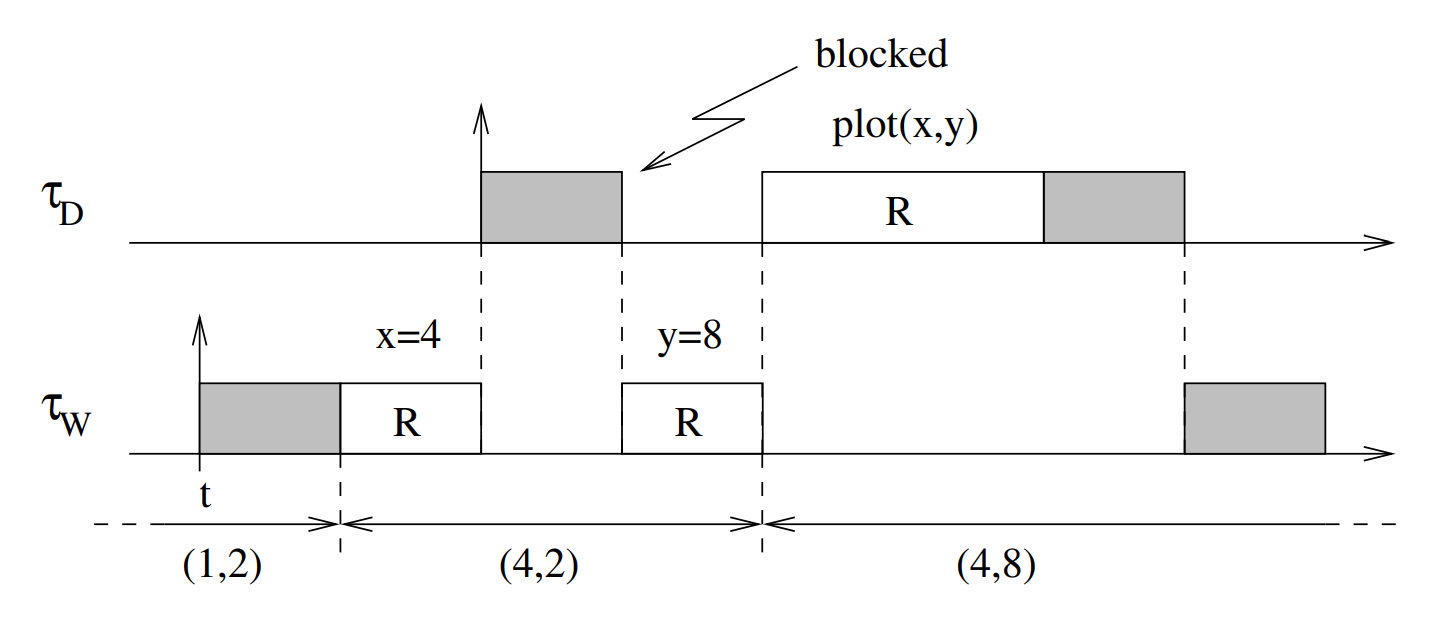
\includegraphics[width=0.5\textwidth]{semaphore}
    \caption{Example of schedule when the resource is protected by a semaphore.. \cite{b5}}
    \label{fig:semaphore}
\end{figure}

\begin{figure}[ht]
    \centering
    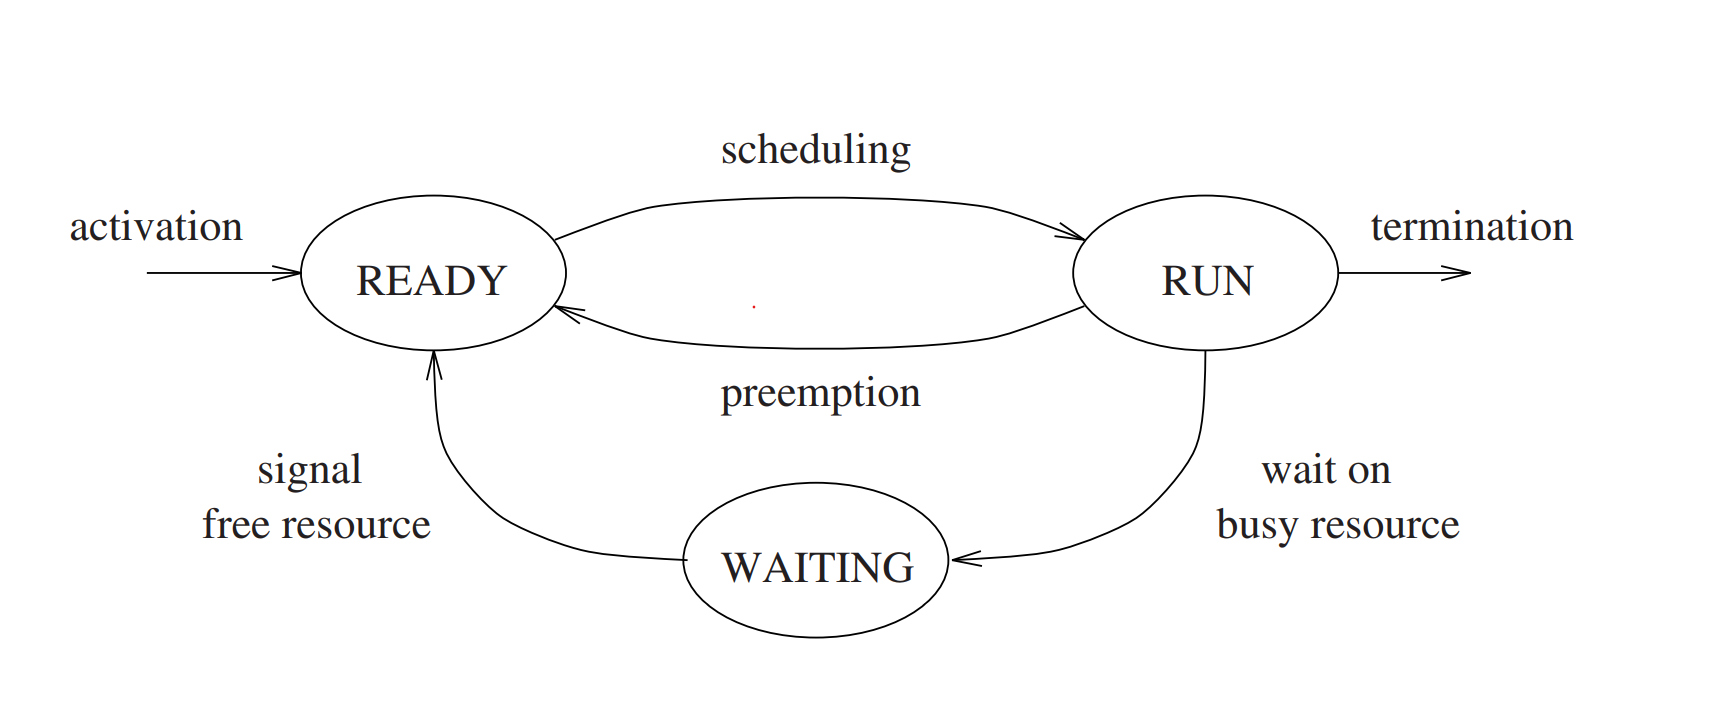
\includegraphics[width=0.5\textwidth]{state}
    \caption{Waiting state caused by resource constraints. \cite{b5}}
    \label{fig:state}
\end{figure}



\subsection{Schedulability}

Before we contemplate implementing a resource access protocol, we must ensure that all tasks are schedulable or that a schedule on the set of tasks is feasible. A scheduability test can be used to accomplish this. The scheduability test will not be discussed in this paper because all tasks are already considered schedulable. \cite{b5} further information on the scheduability test.

In the following section, we'll look at an issue that developed as a result of the suggested synchronization mechanism, which has an impact on the predictability of a real-time system.
%task

%scheduling
%classification
%-preemtion
%-non-preemtion
%-dynamic
%-static
%-online
%periodic
%schedubility test

%constraint
%-timming
%-resource
%share resource
%problem
%solution (resource constarint)

\section{Problem Definition: Invention Priority}

In theory, a set of task that are schedulable will be executed upon on its arriving time and preempted if a task with higher priority arrive. That will not be always true if we apply resource constraint. The problem arrive when a scheduler want to preempt a lower task that is currently accessing a  resource, R and want to execute higher priority task that also want to use the resource. Since the lower priority task didn't yet produce signal(S) primitive where S is the binary semaphore, the higher priority task will be blocked. This phenomenon called priority invention. The implication from this phenomenon is that it will cause unbounded delay on execution of task with higher priority and reduce the predictability of the system because the highest priority task could miss its deadline. The priority invention is illustrated in figure \ref{fig:Example_in_which_NPP_causes_unnecessary_blocking_on_T1} where $ \tau_{1} $ have the highest priority.

Here is where we need resource access protocol to make some adjustment to the scheduler so that the implication of invention priority could be reduced. We're going to discuss this solution in the next sections.
%priority invention


\subsection{Introduction}
\subsection{Model Classification}
\subsection{Terminology and Assumption}
%Introduction
%task
%Model Classification
%Terminology and Assumption
\section{Conclusion}

As the conclusion, Resource access protocol is used in order to maintain the predictability of a real time system by reducing the blocking time experienced by the highest priority task and the most important things is that it help the highest priority task to complete before its deadline to avoid any catastrophic consequence. There are more resources access protocol that can found in \cite{b5} that improves the pervious protocol.


\section*{Acknowledgment}

I would like to express my very great appreciation to Dr Stefan Henkler  for his valuable and constructive suggestions during the planning and development of this research work. His willingness to give his time so generously has been very much appreciated.


\bibliographystyle{plain-annote}

\bibliography{ref} 
\cite{*}
\end{document}
